\documentclass[a4paper,12pt]{book}
\usepackage[utf8]{inputenc}
\usepackage[T1]{fontenc}
\usepackage[english,frenchb]{babel}
\usepackage{a4wide}
\usepackage{mathptmx}
\usepackage{helvet}
\usepackage{listings}
\lstset{basicstyle=\ttfamily, gobble=2}
\usepackage{graphicx}
\graphicspath{{images/}}
\usepackage{hyperref}
\usepackage{color}
\hypersetup{%
  colorlinks=true,
  linkcolor=black,
  citecolor=black,
  urlcolor=black}

\renewcommand{\baselinestretch}{1.05}
\usepackage{fancyhdr}
\pagestyle{fancy}
\fancyfoot{}
\fancyhead[LE,RO]{\bfseries\thepage}
\fancyhead[RE]{\bfseries\nouppercase{\leftmark}}
\fancyhead[LO]{\bfseries\nouppercase{\rightmark}}
\setlength{\headheight}{15pt}

\let\headruleORIG\headrule
\renewcommand{\headrule}{\color{black} \headruleORIG}
\renewcommand{\headrulewidth}{1.0pt}
\usepackage{colortbl}
\arrayrulecolor{black}

\fancypagestyle{plain}{
  \fancyhead{}
  \fancyfoot[C]{\thepage}
  \renewcommand{\headrulewidth}{0pt}
}

\makeatletter
\def\cleardoublepage{\clearpage\if@twoside \ifodd\c@page\else
  \hbox{}%
  \thispagestyle{empty}%
  \newpage%
  \if@twocolumn\hbox{}\newpage\fi\fi\fi}
\makeatother

\usepackage{amsmath}
\usepackage{array}
\usepackage{multirow}
\usepackage[footnote]{acronym}


\parskip=5pt plus2pt minus 1pt
%\sloppy

\frenchbsetup{ReduceListSpacing=false}
\begin{document}

%%%%%%%%%%%%%%%%%%%%%
%%% Page de titre %%%
%%%%%%%%%%%%%%%%%%%%%

\begin{titlepage}
\centering
\sffamily

%%%%%%%%%%%%%%%%%%%%%%%%%%%%%%%%%%%%%%%%%%%%%%%%%
%%% Logos, nom de l'université et de l'entreprise
\begin{minipage}[b]{0.25\linewidth}
  
\includegraphics[width=\linewidth]{logo_dut}
  \par\vspace{2mm}
  \small
  Département\\
  Informatique\\
  IUT Bordeaux 1
\end{minipage}
\hspace{0.25\linewidth}
\begin{minipage}[b]{0.25\linewidth}
  
\includegraphics[width=\linewidth]{logo_y3s}
  \par\vspace{2mm}
  \small
  Société Y3S SAS\\
  47, rue Fragonard\\
  Bruges
\end{minipage}

%%%%%%%%%%%%%%%%%%%
%%% Titre du projet
\vspace{\stretch{1}}
{%
  \bfseries\LARGE
  Solution d'administration à distance d'objets connectés
}

%%%%%%%%%%%%%%%%%%%%%%%%%%%%%%%
%%% Type de mémoire et étudiant
\vspace{\stretch{1}}
Stage de DUT réalisé par\par\medskip
{\Large \bfseries Lorian Corbel}\par\medskip
du 4 avril au 11 juin 2016

%%%%%%%%%%%%%%%%%%%%%
%%% Encadrants projet
\vspace{\stretch{2}}
\renewcommand{\arraystretch}{1.5}
\begin{tabular}{r@{\quad}l}
  Maître de stage & Sylvain \textsc{Leris} \\
  Enseignant responsable & Olivier \textsc{Lys} \\
  Année universitaire & 2015-2016
\end{tabular}
\end{titlepage}

%%%%%%%%%%%%%%%%%%%%%%%%%%%%%
%%% Non-significant pages %%%
%%%%%%%%%%%%%%%%%%%%%%%%%%%%%

\frontmatter

%%%\clearpage

%%%%%%%%%%%%%%%%
%%% Abstract %%%
%%%%%%%%%%%%%%%%

\chapter{Résumé}
\begin{quotation}
  Dans l'univers naissant de l'Internet des objets en plein
  developpement, ces objets hébergent de plus en plus de contenu
  multimédia et service. L'entreprise Y3S recherche une solution pour
  pouvoir accéder à n'importe quel objet connecté à travers internet,
  sans connaître sa configuration réseau actuel ou son adresse
  internet de manière générique.
\end{quotation}

\begingroup
\makeatletter
\renewcommand\chapter{%
  \@afterindentfalse
  \secdef\@chapter\@schapter
}

\begin{otherlanguage}{english}
  \chapter{Abstract}
  \begin{quotation}
    In the nascent world of the Internet of things in full development
    , these objects are home more and more multimedia content and
    services. The company Y3S looking for a solution to access any
    object connected through internet, without knowing its current
    network configuration or IP address generically.
  \end{quotation}
\end{otherlanguage}

\endgroup
% {\textbf{Mots clés :}}
% Lorem ipsum dolor sit amet, consectetur adipiscing elit. Sed non risus. Suspendisse lectus tortor.
% \\
% \noindent\rule[2pt]{\textwidth}{0.5pt}
% \begin{center}
%   ISAE\\
%   10, avenue Édouard Belin\\
%   BP 54032\\
%   31055 Toulouse CEDEX 4
% \end{center}
% \vspace*{\fill}

\chapter{Remerciements}
Je tiens à remercier Sylvain \textsc{Leris}, mon maître de stage, pour m'avoir accepté dans l'entreprise et accompagné pendant toute la durée de mon stage. Je remercis également Yann \textsc{Garras} pour toute l'aide et conseils qu'il a pu m'apporter.

Pour terminer je remercis Olivier \textsc{Lys}, mon professeur référent et toute l'équipe pédagogique du département informaque de l'IUT de Bordeaux pour ces deux années de DUT.

%%% \clearpage
\tableofcontents

%%% \clearpage
\listoffigures

%%% \clearpage
\chapter{Liste des sigles et acronymes}
\begin{acronym}[CP-OFDMX] % Give the longest acronym here
\acro{IP}{\emph{Internet Protocol}}
\acro{TCP}{\emph{Transmission Control Protocol}}
\acro{HTTP}{\emph{HyperText Transfer Protocol}}
\acro{MIPS}{\emph{Microprocessor Without Interlocked Pipeline Stages}}
\acro{RISC}{\emph{Reduced Instruction Set Computer}}
\acro{CISC}{\emph{Complex Instruction Set Computer}}
\acro{GCC}{\emph{GNU Compiler Collection}}
\acro{VPN}{\emph{Virtual Private Network}}
\acro{SSH}{\emph{Secure Shell}}
\acro{SSL}{\emph{Secure Sockets Layer}}
\acro{TLS}{\emph{Transport Layer Security}}
\acro{RAM}{\emph{Random Access Memory}}
\acro{IOT}{\emph{Internet Of Things}}
\acro{SDK}{\emph{Software Development Kit}}
\acro{SIG}{\emph{Système Informatique Géographique}}
\end{acronym}

%%%%%%%%%%%%%%%%%%%%%%%%%%%%%%%%%%%%%%%%%%%%
%%% Content of the report and references %%%
%%%%%%%%%%%%%%%%%%%%%%%%%%%%%%%%%%%%%%%%%%%%

\mainmatter
\pagestyle{fancy}

%%% \cleardoublepage

\chapter*{Introduction}
\addcontentsline{toc}{chapter}{Introduction}
\markboth{Introduction}{Introduction}
\label{chap:introduction}
%\minitoc

Lorem ipsum dolor sit amet, consectetur adipiscing elit. Sed non risus. Suspendisse lectus tortor, dignissim sit amet, adipiscing nec, ultricies sed, dolor. Cras elementum ultrices diam. Maecenas ligula massa, varius a, semper congue, euismod non, mi. Proin porttitor, orci nec nonummy molestie, enim est eleifend mi, non fermentum diam nisl sit amet erat. Duis semper. Duis arcu massa, scelerisque vitae, consequat in, pretium a, enim. Pellentesque congue. Ut in risus volutpat libero pharetra tempor. Cras vestibulum bibendum augue. Praesent egestas leo in pede. Praesent blandit odio eu enim. Pellentesque sed dui ut augue blandit sodales. Vestibulum ante ipsum primis in faucibus orci luctus et ultrices posuere cubilia Curae; Aliquam nibh. Mauris ac mauris sed pede pellentesque fermentum. Maecenas adipiscing ante non diam sodales hendrerit. Ut velit mauris, egestas sed, gravida nec, ornare ut, mi. Aenean ut orci vel massa suscipit pulvinar. Nulla sollicitudin. Fusce varius, ligula non tempus aliquam, nunc turpis ullamcorper nibh, in tempus sapien eros vitae ligula. Pellentesque rhoncus nunc et augue. Integer id felis. Curabitur aliquet pellentesque diam. Integer quis metus vitae elit lobortis egestas. Lorem ipsum dolor sit amet, consectetuer adipiscing elit. Morbi vel erat non mauris convallis vehicula. Nulla et sapien. Integer tortor tellus, aliquam faucibus, convallis id, congue eu, quam. Mauris ullamcorper felis vitae erat. Proin feugiat, augue non elementum posuere, metus purus iaculis lectus, et tristique ligula justo vitae magna. Aliquam convallis sollicitudin purus. Praesent aliquam, enim at fermentum mollis, ligula massa adipiscing nisl, ac euismod nibh nisl eu lectus. Fusce vulputate sem at sapien. Vivamus leo. Aliquam euismod libero eu enim. Nulla nec felis sed leo placerat imperdiet. Aenean suscipit nulla in justo. Suspendisse cursus rutrum augue. Nulla tincidunt tincidunt mi. Curabitur iaculis, lorem vel rhoncus faucibus, felis magna fermentum augue, et ultricies lacus lorem varius purus. Curabitur eu amet.

Lorem ipsum dolor sit amet, consectetur adipiscing elit. Sed non risus. Suspendisse lectus tortor, dignissim sit amet, adipiscing nec, ultricies sed, dolor. Cras elementum ultrices diam. Maecenas ligula massa, varius a, semper congue, euismod non, mi. Proin porttitor, orci nec nonummy molestie, enim est eleifend mi, non fermentum diam nisl sit amet erat. Duis semper. Duis arcu massa, scelerisque vitae, consequat in, pretium a, enim. Pellentesque congue. Ut in risus volutpat libero pharetra tempor. Cras vestibulum bibendum augue. Praesent egestas leo in pede. Praesent blandit odio eu enim. Pellentesque sed dui ut augue blandit sodales. Vestibulum ante ipsum primis in faucibus orci luctus et ultrices posuere cubilia Curae; Aliquam nibh. Mauris ac mauris sed pede pellentesque fermentum. Maecenas adipiscing ante non diam sodales hendrerit. Ut velit mauris, egestas sed, gravida nec, ornare ut, mi. Aenean ut orci vel massa suscipit pulvinar. Nulla sollicitudin. Fusce varius, ligula non tempus aliquam, nunc turpis ullamcorper nibh, in tempus sapien eros vitae ligula. Pellentesque rhoncus nunc et augue. Integer id felis. Curabitur aliquet pellentesque diam. Integer quis metus vitae elit lobortis egestas. Lorem ipsum dolor sit amet, consectetuer adipiscing elit. Morbi vel erat non mauris convallis vehicula. Nulla et sapien. Integer tortor tellus, aliquam faucibus, convallis id, congue eu, quam. Mauris ullamcorper felis vitae erat. Proin feugiat, augue non elementum posuere, metus purus iaculis lectus, et tristique ligula justo vitae magna. Aliquam convallis sollicitudin purus. Praesent aliquam, enim at fermentum mollis, ligula massa adipiscing nisl, ac euismod nibh nisl eu lectus. Fusce vulputate sem at sapien. Vivamus leo. Aliquam euismod libero eu enim. Nulla nec felis sed leo placerat imperdiet. Aenean suscipit nulla in justo. Suspendisse cursus rutrum augue. Nulla tincidunt tincidunt mi. Curabitur iaculis, lorem vel rhoncus faucibus, felis magna fermentum augue, et ultricies lacus lorem varius purus. Curabitur eu amet.

%%% Local Variables: 
%%% mode: latex
%%% TeX-master: "isae-report-template"
%%% End: 

\chapter{L'entreprise}
\label{chap:y3s}

\section{Y3S SAS, une ESN polyvalente}

\subsection{Organisation}
La société Y3S est une Société par Actions Simplifiée, fondé il y a deux ans par ses deux associés, Sylvain \textsc{Leris} et Yann \textsc{Garras}. Ils rassemblent à eux deux des compétences variés dans le domaine du WEB (Node.js, PHP, Javascript, AngularJS, JEE), mobile (iOS, android, cordova), embarqué (Buildroot, kernel unix, ARM, C/C++, C\#), Système Informatique Géographique (base de données spatial, QGIS).


Aujourd'hui la société emploie toujours deux personnes :
\begin{itemize}
    \item Sylvain \textsc{Leris} : Président
    \item Yann \textsc{Garras} : Directeur Général
\end{itemize}

La société fonctionne sur un modèle économique en deux branches principales :
\begin{itemize}
    \item Prestation de services : développement d'application WEB, mobile ou embarqué pour des clients en fonction de la demande.
    \item Editeur de solution : développement de solution propre à la société, comme par exemple une bibliothèque de Système Informatique Géographique.
    \item Formation : bien qu'elle soit moins présente, c'est une activité possible de la société, mais uniquement sur des formation spécifique. 
\end{itemize}

Sur tout ce qui est prestation de service et editeur de solution, Y3S SAS cherche à obtenir une continuité de maintenance avec leur client.

%%% Local Variables: 
%%% mode: latex
%%% TeX-master: "isae-report-template"
%%% End: 

\chapter{Solution d'administration à distance d'objets connectés}
\label{sec:content}

\section{Nécéssité de cette solution}

La société Y3S developpe toute sorte d'objets connectés comme des centrales d'alarmes, sondes de relevé de température et tous hébergent un serveur HTTP local pour sa gestion ou son utilisation malheureusement pour accéder à son contenu local depuis internet il faut ouvrir les ports et configurer les routeurs sur lequel j'y est connecté l'objet. Pour les grandes entreprises ou collectivités il n'est pas toujours possible d'effectuer ce genre de modification à leur architecture réseau à cause de problèmes de sécurité, de compétence ou tout simplement parce que le nombre d'objets connectés est trop important pour recevoir ces configurations manuellement pour chaque unité.

Une autre solution consiste à developper un CLOUD sur lequel se connectent tout les objets connectés et permettant aux utilisateurs d'y accéder par l'intermédiaire d'un frontend HTTP par exemple. Cette solution reste extrêmement couteuse, en effet elle nécessite de développer une solution CLOUD spécifique à chaque service ou type d'objet connecté.

C'est donc dans cette optique que l'entreprise recherche une solution qui permet de remplacer le CLOUD par une solution plus générique qui donnerait directement accès aux services locaux hébergés directement sur l'objet connecté, réduissant ainsi les coût en developpement et installation.

\section{Spécifications}

\subsection{Spécifications fonctionnelles}

Il est necessaire de développer la solution en deux partie, le client a installé sur l'objet et le serveur backend en charge de rendre l'objet connecté accesible sur internet. La solution doit être capable de fournir un client ou un SDK à installer sur l'objet connecté, qui permet de se connecter au serveur backend de la solution. Les principales fonctionnalités de la solution sont :

\begin{itemize}
    \item Générer un nom de domaine unique par objet connecté qui hébergent un serveur HTTP.
    \item Gérer les déconnexions, reconnexions de l'objet connecté, pointer sur une page HTML d'erreur si on tente d'accéder au nom de domaine d'un objet déconnecté et founir un nouveau nom de domaine unique si l'objet est resté deconnecté jusqu'à l'écoulement d'un délai prédéfini, sinon lui resservir le même nom de domaine.
    \item Pouvoir se reconnecter automatiquement à un des serveurs s'il perd la connexion.
    \item La solution ne doit pas se contenter d'un seul protocole tel que le HTTP, mais doit pouvoir relayer n'importe quel protocole utilisant le TCP.
\end{itemize}

\subsection{Contraintes}

Le monde des objets connectés utilise des architectures de processeur spécifiques et variés. La solution cliente doit donc être multi-plateforme, elle doit fonctionner sur UNIX, Windows, Android sur des architectures x86/x64, ARM, MIPS. On doit pouvoir aussi réimplémenter le client sur microcontrôleur possédant une stack IP parce qu'il sont très utilisés dans le monde de l'industrie et donc des objets connectés.

Certaine entreprise ont des pare-feux très restrictifs ne permettant la sortie que de certain protocole comme le HTTP et HTTPS respectivement sur le port 80 et 443.

\subsection{Spécifications techniques}

Pour répondre aux besoins de la solution, des choix techniques ont étés fait tout le long du developpement du prototype de la solution. Au début Y3S m'a demandé de comparer les solutions existantes de Reverse Tunneling, qui leur semblait être la technique la plus pertinente, particulièrement si la solution utilise les websockets.

J'ai personnellement choisi de développer le client en C++, un langage bas niveau orienté objet qui reste facile à compiler sur plusieurs architectures. Le serveur a été développé en nodejs pour sa simplicité de mise en place et de developpement, sa scabilité et sa maintenance.

Pour résumer, voici les technologies techniques utilisés actuellement sur le prototype à la fin de son développement, leur justification d'utilisation suivra dans le rapport :

\begin{itemize}
    \item Reverse Tunneling en websocket : transfert de protocole TCP à travers n'importe quel routeur, pare-feu qui accepte le HTTP/HTTPS.
    \item C++ et socket natif : développement client.
    \item Node.js : développement serveur.
    \item Redis : base de données.
    \item OpenResty : proxy HTTP dynamique.
\end{itemize}

\section{Principe du Reverse Tunneling}

Pour illustrer le principe du reverse tunneling je vais me servir d'un scénario. Imaginons que je souhaite atteindre le serveur HTTP d'Alice, mais Alice est derrière un NAT qui bloque toute les connexions entrantes sur son réseau. Malheureusement elle n'a pas la main sur son routeur, ce qui empêche naturellement toute modification du réseau. Par contre Bob a le contrôle de son réseau, qui accepte les connexions entrante sur sa machine, ce qui va me permettre de procéder en sens inverse. C'est Alice que je souhaite joindre qui va créer une connexion vers Bob que j'appelle le tunnel. En effet il suffit à Bob d'écouter sur le port de son choix qu'Alice connait, il attend qu'Alice se connecte dessus et lui transmet sa requête HTTP. De son côte Alice va recevoir la requête HTTP de Bob, qu'elle relaye à son serveur HTTP et renvoit la réponse HTTP par cette même connexion. C'est pour cela que cela s'appelle du reverse tunneling, c'est notre cible qui est à l'initiative de la connexion, autrement dit du tunnel.

\section{Comparaison de solution de reverse tunnel}

Après quelque jours de recherche, j'ai retenu trois solutions de reverse tunnel :

\begin{itemize}
    \item OpenSSH
    \item Etherws
    \item Node Reverse Wstunnel
\end{itemize}

\subsection{OpenSSH}

OpenSSH est une suite d'outils SSH libre mettant à disposition un client et server SSH très complet. Hors le SSH permet d'initialiser un tunnel directement avec une commande SSH. Pour en revenir sur notre scénario précédent. Bob installe un serveur SSH sur sa machine (en 22), toujours accessible de l'extérieur par le nom de domaine bob.fr et rajoute sur son serveur SSH l'utilisateur alice. Elle va s'y connecter en précisant qu'elle ouvre un tunnel inverse de son port 80 sur lequel écoute son serveur HTTP, jusqu'au port de son choix par exemple le 8080. Bob peut desormais accéder au serveur d'Alice en remontant le tunnel par l'adresse http://localhost:8080.

 L'action se résume par cette unique ligne de commande qu'Alice exécute sur sa machine :
\begin{lstlisting}[language=bash]
  $ ssh -NR 8080:localhost:80 alice@bob.fr
\end{lstlisting}%$

Bien évidemment cela fonctionne pour n'importe quel service en TCP, il suffit juste de choisir le bon port.

Avantages :
\begin{itemize}
    \item Facile à mettre en place.
    \item Automatiquement sécurisé.
\end{itemize}

Inconvénients :
\begin{itemize}
    \item Les microcontrôleur ne possèdent pas de client SSH, en développer un serait périlleux.
    \item Pour chaque port ouvert il faut une nouvelle connexion SSH.
    \item Un serveur SSH n'est pas optimisé pour maintenir une centaine de connexion permanente.
    \item Le port d'entrée et sortie du tunnel est choisi par le client.
    \item Puisque que cest du SSH, le port du serveur tunnel y est auss.
\end{itemize}

\subsection{Etherws}

Etherws est un mini VPN utilisant des websockets comme tunnel, il est entièrement développé en python. La configuration se fait en deux étapes, d'abord la création de l'interface virtuelle en TUN/TAP avec l'adressage de l'IP virtuelle, puis la connexion au serveur (toujours celui de Bob qui est le seul à disposé d'un nom de domaine public). Le fait d'utiliser une interface virtuelle permet d'utiliser tous les ports à la fois sans en préciser un en particulier qui doit être relié à un autre distant sur la machine de Bob.

Dans notre cas Alice va choisir d'appeler son interface virtuel \og etherws0 \fg{} avec l'IP \og 10.0.2.8 \fg{} et se connecter sur le serveur etherws de Bob (en 80). Pour accéder au serveur HTTP d'Alice, Bob doit remonter le tunnel en passant par l'IP virtuele d'Alice, soit comme cela http://10.0.2.8:80.

 Commande nécessaire à la création du tunnel :
\begin{lstlisting}[language=bash]
  etherws sw
  etherws ctl addport tap ethws0
  etherws ctl setif --address 10.0.2.8 --netmask 255.255.255.0 1
  etherws ctl addport client ws://bob.fr/
\end{lstlisting}

Avantages :
\begin{itemize}
    \item Utilise les websockets.
    \item Peut être sécurisé en SSL/TLS.
\end{itemize}

Inconvénients :
\begin{itemize}
    \item Monte une interface virtuelle.
    \item L'IP virtuelle est choisi par le client.
    \item Tous les clients peuvent communiquer ensemble par le réseau virtuel.
    \item Portage difficile, voir impossible sur microcontrôleur.
\end{itemize}

\subsection{Node Reverse Wstunnel}

Node Reverse Wstunnel est un tunnel inversé développé en javascript avec Node.js, utilisant les websockets. Il s'utilise sur le même principe que le tunnel inversé SSH mais en passant par un tunnel websocket au lieu d'un tunnel SSH. Bob lance sur sa machine le serveur tunnel inversé en 80 (avec node) et Alice s'y connecte avec le client fourni en précisant les deux ports qu'elle veut relier.

Si on reprend la même configuration que pour le tunnel SSH, la commande qu'Alice doit exécuter est :
\begin{lstlisting}[language=bash]
  $ ./wstt.js -r 8080:localhost:80 ws://bob.fr/
\end{lstlisting}%$

Bob peut donc accéder au serveur HTTP d'Alice en se connectant en http://localhost:8080.

Avantages :
\begin{itemize}
    \item Utilise les websockets.
    \item Peut être sécurisé en SSL/TLS.
\end{itemize}

Inconvénients :
\begin{itemize}
    \item Le port d'entrée et sortie du tunnel est choisi par le client.
\end{itemize}

\subsection{Choix final}

Finalement j'ai décidé avec mon maître de stage de choisir la solution de reverse tunneling en Node.js en websocket, mais en reprogrammant le client en C++ parce que le Node.js n'est pas portable sur toute les versions d'ARM. Le serveur restera en Node.js mais sera re-écris pour mieux répondre à nos besoins, c'est en effet une technologie facilement maintenable pour développer un serveur websocket évolutif. L'architecture de base de Node Reverse Wstunnel est la seule chose conservée dans son intégrité.

\section{Proxy HTTP dynamique}

J'ai résolu comment accéder à une machine distante sans modifier son NAT ou connaître son IP. Cependant notre objectif est d'accéder à plusieurs machines, objets connectés à travers un nom de domaine unique pour chaque. Actullement si je reprends l'exemple précédent d'Alice et Bob. Alice fait tourner son serveur HTTP sur le port 80, en se connectant au serveur wstunnel de Bob, elle a demandé à relier son port 80 avec le port 8080 de Bob. Ainsi depuis internet, si on se connecte en http://bob.fr:8080 on accéde au serveur HTTP d'Alice, car Bob possède un nom de domaine qui pointe sur l'IP fixe de sa machine. Cela fonctionne parfaitement sauf qu'on voulait un nom de domaine sans devoir préciser le port, certes on pourrait déplacer le serveur wstunnel sur le port 8080 et remettre le tunnel du port 80 d'Alice au port 80 de Bob comme cela le nom de domaine serait bob.fr tout simplement. Mais qu'arriverait il si je souhaite rajouter une ou dix autre machine dans le même cas qu'Alice ? Il me faudrait bien utiliser des ports autre que le 80.

C'est pour résoudre ce problème que j'ai dû installer un proxy HTTP. Celui-ci est en fait un serveur HTTP qui va rediriger une requête ou une réponse HTTP sur un autre port en fonction du nom de domaine. Quand je rentre un nom de domaine dans un navigateur, celui-ci va résoudre le nom de domaine en IP et envoyer une requête HTTP sur cette IP, port 80 par défaut. C'est grâce à la requête HTTP que le proxy peut connaître le serveur cible sur lequel rediriger la requête. En effet une requête HTTP contient un champs \og Host \fg{} qui contient le nom de domaine que l'utilisateur a saisi dans le navigateur, le proxy redirige donc en fonction de ses configurations sur tel ou tel port la requête et la réponse HTTP.

Dans ce cas Bob peut configurer son proxy HTTP qui écoute sur le port 80 de rediriger le nom de domaine \og alice.bob.fr \fg{} en \og localhost:8080 \fg{} (le serveur wstunnel est sur un autre port disponible).

Exemple de requête HTTP :
\begin{lstlisting}[language=bash]
  GET / HTTP/1.1
  Host: alice.bob.fr
\end{lstlisting}

Malheureusement la plupart des proxy HTTP sont configurables à l'arrêt, ce qui veut dire que si je veux rediriger d'autre serveur HTTP comme Alice, je dois éditer les configurations du proxy et redémarrer les services, le tout manuellement, ce qui est tout simplement impossible pour les objectifs de la solutions de pouvoir rediriger des centaines de nom de domaines uniques pour autant d'objets connectés. Il m'a fallu rechercher un solution dynamique à notre problème.

OpenResty est un serveur, proxy HTTP basé sur Nginx, qui a la particularité d'être très modulables grâce à ces nombreux modules configurables et à la possibilité d'exécuter des scripts LUA lorsque l'on reçoit une requête HTTP. LUA est un langage de scripting très léger et facile à embarquer. Avec OpenResty j'ai pu écrire une configuration de proxy qui lorsque qu'il reçoit une requête, recherche \og Host \fg{} dans notre base de données et si ce nom de domaine existe dans la base, alors redirige la requête vers l'IP et port associés. Tout cela est possible grâce à un script LUA qui se connecte à la base de données, de plus je peux rajouter des noms de domaines à rediriger dans la base de données sans à devoir redémarrer le proxy. OpenResty m'a donc permis de créer un proxy HTTP dynamique.

\section{Base de données Redis}

Pour faire fonctionner l'ensemble de la solution, il a fallut faire le choix d'une base de données centrale qui ferait le lien entre le proxy HTTP dynamique et le serveur wstunnel en Node.js, mais aussi avec la futur partie front-end, en charge d'afficher la liste des ports redirigés pour chaque client et le nom de dommaine unique si c'est un port 80 ou 443. J'ai fait le choix d'utiliser Redis, qui est une base de données No-SQL dont la particularité est de stocker tout son contenu dans la mémoire vive. Redis utilise des structures de données très simple comme des listes, des ensembles, des tableaux associatifs ou même des ensembles triés. Elle peut en stocker des dizaines de millions de clefs et valeurs dans à peines 100 Mio de RAM. Son protocole de communication, ses structures et son stockage en RAM ont fait d'elle une base de données extrement rapide, c'est justement ce qu'il faut pour que notre proxy HTTP dynamique réponde le plus rapidement possible aux requêtes. Une petite fonctionnalité de Redis permet aussi de rajouter un délai d'expiration sur certaines valeurs stockées avant leur suppression, cela s'est avérait pratique pour supprimer automatiquement les noms de domaines et ports qui n'etaient plus utilisés par l'objet connecté qui s'est justement déconnecté. Une fonctionnalité qui permet donc de libérer les ports non utlisés et regagner en capacité. Par contre si l'objet connecté se reconnecte avant la fin du délai, alors il conserve son port et son nom de domaine alloué. Si jamais le serveur tombe et que l'on perd les données Redis stockés dans la RAM, cela n'est pas très grave, les données en questions sont les ports et les nom de domaine qui étaient utilisés par le serveur tunnel, mais si Redis est tombé alors le serveur tunnel l'est aussi donc tout ses ports utilisés ne sont plus du tout d'actualités.

\section{Modification et Re-developpement du Tunnel WebSocket}

\subsection{WebSocket}

Le websocket est un protocole réseau standard du Web visant à créer une communication full-duplex sur une connexion HTTP, donc en TCP. Ce protocole a été normalisé dans la RFC 6455, son but est de pouvoir établir des communications bidirectionnelles avec un long temps de vie entre le client et serveur HTTP afin de notifier le client d'un changement d'état du serveur ou même d'envoyer des données ponctuelles du serveur au client.

Pour initialiser une connexion websocket il faut envoyer une requête HTTP spécifique au serveur qu'on appelle le \og Handshake \fg{} au quel le serveur doit répondre avec une réponse HTTP. Ensuite à partir de cette échange, la connexion HTTP passe en connexion websocket.

Exemple de requête handshake :
\begin{lstlisting}[language=bash]
  GET /chat HTTP/1.1
  Host: example.com:8000
  Upgrade: websocket
  Connection: Upgrade
  Sec-WebSocket-Key: dGhlIHNhbXBsZSBub25jZQ==
  Sec-WebSocket-Version: 13
\end{lstlisting}

Exemple de réponse handshake :
\begin{lstlisting}[language=bash]
  HTTP/1.1 101 Switching Protocols
  Upgrade: websocket
  Connection: Upgrade
  Sec-WebSocket-Accept: s3pPLMBiTxaQ9kYGzzhZRbK+xOo=
\end{lstlisting}

Lors du handshake le client passe dans la requête HTTP le champs \og Sec-WebSocket-Key \fg{} qui contient une clef aléatoirement générée par le client et cryptée en base64. Le serveur doit hasher en SHA1 la concaténation de cette clef avec une chaîne de caractère prédéfini dans la RFC 6455 et convertir la sortie en base64, ce qui correspond dans la réponse au champs \og Sec-WebSocket-Accept \fg{}. Le client doit ou peut réaliser la même opération pour vérifier qu'il communique bien avec un serveur websocket et non un proxy qu'il lui renverrait un simple cache.

La suite de la communication est entièrement basée sur des trames websocket binaires, rythmés par des échanges de trames de controle ping et pong dit \og battement de coeur \fg{}, pour avoir la certitude que le la connexion est toujours active. Je ne vais pas détailler d'avantage les trames websocket car cela est peu utile et très spécifique, il suffit de lire la RFC 6455, je rajouterai seulement que le webscoket permet d'envoyer deux type de données, du texte brute UTF-8 et du binaires.

\begin{figure}[htp]
\centering
\begin{lstlisting}[gobble=0, numbers=left, frame=l,
  basewidth={0.55em, 0.4em}]
 0               1               2               3              
 0 1 2 3 4 5 6 7 0 1 2 3 4 5 6 7 0 1 2 3 4 5 6 7 0 1 2 3 4 5 6 7
+-+-+-+-+-------+-+-------------+-------------------------------+
|F|R|R|R| opcode|M| Payload len |    Extended payload length    |
|I|S|S|S|  (4)  |A|     (7)     |             (16/64)           |
|N|V|V|V|       |S|             |   (if payload len==126/127)   |
| |1|2|3|       |K|             |                               |
+-+-+-+-+-------+-+-------------+ - - - - - - - - - - - - - - - +
 4               5               6               7              
+ - - - - - - - - - - - - - - - - - - - - - - - - - - - - - - - +
|     Extended payload length continued, if payload len == 127  |
+ - - - - - - - - - - - - - - - +-------------------------------+
 8               9               10              11             
+ - - - - - - - - - - - - - - - +-------------------------------+
|                               |Masking-key, if MASK set to 1  |
+-------------------------------+-------------------------------+
 12              13              14              15
+-------------------------------+-------------------------------+
| Masking-key (continued)       |          Payload Data         |
+-------------------------------- - - - - - - - - - - - - - - - +
:                     Payload Data continued ...                :
+ - - - - - - - - - - - - - - - - - - - - - - - - - - - - - - - +
|                     Payload Data continued ...                |
+---------------------------------------------------------------+
\end{lstlisting}
\caption{Trame WebSocket}
\end{figure}

\subsection{Fonctionnement}

Pour expliquer le principe de fonctionnemment du tunnel en websocket (qui sera toujours en mode \og reverse \fg{}) qu'on applera plus facilement le tunnel, sans pour l'instant y ajouter le proxy HTTP dynamque, je vais en rédéfinir les acteurs, il y en a trois principaux :
\begin{itemize}
    \item Le serveur, c'est le serveur websocket principal qui pilote tout le tunnel, son IP est donc connu et publique. Il est connectés à la base de données Redis, sur laquel il stock les ports alloué et connexions courantes.
    \item Le client, c'est la machine ou objet connecté souhaitant rendre accessible un de ses serveurs au public, dans notre cas se sera un serveur HTTP.
    \item Le navigateur, c'est un utilisateur externe qui veut accéder au service du client, dans notre cas il fait une requête HTTP sur un port défini du serveur websocket. 
\end{itemize}

Pour faire fonctionner le tunnel il faut au minimum deux connexions websocket, la première est le websocket de contrôle, il sert à initialiser et avertir le client d'une nouvelle connexion du navigateur. Dans le handshake du websocket de contrôle, il faut passer dans l'URL les paramètres suivant, le nom du client et les ports qu'il souhaite faire passer. Le serveur va allouer au client un port disponible sur sa machine ou bien lui donner un port qu'il a déjà utilisé lors de sa précédente connexion mais qui n'a pas encore expiré. Le serveur va monter ce nouveau port alloué comme serveur TCP et y attendre une connexion. Bien sur si un client avec le même nom est déjà connecté la connexion sera refusé. C'est ce que j'appelle la phase d'initialisation du tunnel. Maintenant un navigateur qui connait le port alloué au client sur le serveur va se connecter dessus et y effectuer une requête HTTP. Le serveur va accepté la connexion étant donné qu'une requête HTTP utilise le TCP, il va mettre en attente le navigateur, tagger cette connexion avec un ID unique et envoyer un message sur le websocket de contrôle au client associé à ce port alloué. Ce message est très simple, il contient simplement le port qui a été associé à cette allocation de port lors de la phase d'initialisation du tunnel, soit le port 80 pour un serveur HTTP et l'ID de la connexion du navigateur. En recevant ce message par le websocket de contrôle le client va créer un nouvelle connexion websocket sur le serveur, que j'appelle le websocket de transfert, mais cette fois l'URL du handshake contiendra en paramètre l'ID associé à la connexion du navigateur. Il va aussi créer une connexion locale vers son serveur HTTP et la relier au nouveau websocket de transfert, parce que le message reçu indiqué une redirection sur le port 80. Ainsi le serveur quand il va recevoir la connexion websocket saura exactement que c'est un websocket de transfert grâce à l'ID dans l'URL associé à la connexion du navigateur en cours. Maintenant que le tunnel est completement formé le serveur va rediriger la requête du navigateur dans le websocket de transfert associé en mode binaire, qui va lui même la rediriger côté client au serveur HTTP. Celui-ci va répondre en envoyant une réponse HTTP qui va faire le chemin inverse. Une fois la réponse arrivée jusqu'à son destinataire, le navigateur va fermer la connexion TCP, ce qui va fermer également le websocket de transfert associé à cette connexion ainsi que la connexion local au serveur HTTP du client. Seul restera le websocket de contrôle et le serveur TCP monté sur le port alloué, qui attendront une nouvelle connexion d'un navigateur. Du fait que les connexions du navigateur soient taggées d'un ID unique, plusieurs connexions peuvent être traitées à la fois, ce qui entraine autant de websocket de transfert que de connexions des navigateurs, voilà pourquoi le websocket de contrôle n'est là que pour avertir des nouvelles connexions et ne fait pas aussi le transfert des requêtes. Si c'était le cas il y aura trop d'attente entre chaque requête. Lorsque que le client va fermer la connexion du websocket de contrôle alors le serveur TCP associé au port alloué au client va se fermer et le port prendra un délais d'expiration dans la base de données Redis.

\subsection{Répartition de la charge}

Cette solution serveur tunnel est prévus pour accueillir des centaines ou millier de client. Chaque client doit au minimum maintenir avec le serveur une connexion websocket de contrôle permanente, parce qu'un serveur ne doit enprincipe jamais s'éteindre. Ce qui pose un problème de capacité machine, en effet une machine physique ne peut ouvrir qu'un certain nombre de port maximum, notre serveur tunnel doit donc être multiplié en plusieurs grappes.

Pour palier à ce problème j'ai rajouté une petite implémentation sur le serveur tunnel, chaque serveur dispose d'une IP et d'un compteur de client dans la base de données Redis. Quand un client ce connecte sur un serveur, celui-ci va faire un requête à Redis pour trier et selectionner l'IP qui possède le moins de client grâce au compteur de chaque serveur. Si l'IP qu'il obtient est la sienne, alors le serveur tunnel accepte la connexion websocket de contrôle et incrémente son compteur, sinon il retourne au client une réponse HTTP de code 302 avec en location l'IP, ce qui signifit une redirection HTTP sur cette IP, ne pas oublier que le websocket est construit sur un serveur HTTP à l'aide d'une requête handshake donc c'est totalement possible. Le client va devoir refaire une connexion websocket sur l'IP de redirection, jusqu'a obtenir un serveur qui l'accepte.

\section{Le client}

\subsection{Toolchain}

j'ai choisi de développer le client en C++, ce qui m'a demandé de compiler le client pour chaque architectures. J'ai donc dû faire de la compilation croissée en utilisant une chaîne de compilation (\og toolchain \fg{}) spécifique, c'est-à-dire que j'ai compilé sous UNIX mais en utilisant un compilateur qui a compilé mes sources dans un format d'exécutable, qui pouvait être exécuté que sur le système d'exploitation et architectures cible. Toute ces chaînes de compilations avaient en commun d'être basée sur le compilateur GCC. J'ai utilisé ces chaînes de compilation pour ces cibles précise :
\begin{itemize}
    \item arm-linux-gnueabi : pour ARM (Android, Raspbian et autre kernel UNIX).
    \item mips-openwrt-linux-uclibc : pour MIPS (Arduino Yun).
    \item x86\_64-w64-mingw32 : pour Windows x64.
    \item i686-w64-mingw32 : pour Windows x32, particulièrement Windows XP.
\end{itemize}

Certaine chaîne de compilation ont dû elle même être compilé pour être éxécuté sur ma version de GNU/Linux de développement.

\subsection{Socket natif}

Pour m'assurer d'être entièrement portable j'ai essayé de ne pas utilisé de bibliothèque tiers. J'ai seulement utilisé une bibliothèque de cryptographie pour pouvoir vérifier la validité de la clef du hanshake websocket renvoyé par le serveur. Elle m'a permet d'utiliser le SHA1 et la base64, mais à cause de cela, je l'ai re-compilé à la main, en ré-écrivant les makefiles pour chaque architecture ce qui était plustôt fastidieux.

Puisque que je n'utilisais pas de bibliothèque réseau, j'ai directement utilisé les sockets natif à chaque système d'exploitation. Les sockets permettent de réaliser facilement des connexions TCP ou UDP ou d'ouvrir un port pour y attendre des connexions. Ce sont des fonctionnalités réseau assez bas niveau, j'ai dû écrire par dessus ma propre implémentation d'un client websocket et d'un proxy de redirection de flux. Malheureusement les sockets sont encore une fonctionnalités pas completement portable. En effet certaines fonctionnalités liés aux sockets sont différentes sur UNIX et sur Windows, voir même inexistante sur d'autre.

Pour palier à ce problème, j'ai utilisé des MACRO conditionnels en C, pour que mon compilateur me compile une partie de mon code source uniquement pour un systèmes d'exploitation et pas pour les autres. Pour les fonctionnalités inexistantes, je n'ai pas eu le choix que de l'ai remplacé par d'autre plus ancienne, c'est le cas avec Windows XP qui n'avait pas des fonctions essentiels de gestion de socket existante sur windows Vista, Seven ou 10.

Etant donné que le client doit pouvoir lire plusieurs sockets en même temps, quand par exemple plusieurs connexion websocket de transfert sont créés. J'ai utilisé des sockets en mode asynchrone, c'est-à-dire qu'ils ne bloquaient pas le processus quand ils n'avaient rien à recevoir d'une connexion. Cela nécessite d'utiliser aussi des fonctions systèmes de gestion de sockets qui ne consomme pas de CPU quand il n'y a rien à recevoir. J'ai par exemple utilisé \og poll \fg{}, appelé \og WSAPoll \fg{} sous windows, qui servait à me signaler quand il y avait un socket possible à lire parmis un tableau de sockets. Sous windows XP \og WSAPoll \fg{} n'existe pas, j'ai utilisé une autre version plus ancienne appelé \og select \fg{}. Toute ces modifications spécifiques ont pu être possible sur le même code source en utilisant les MACROs conditionnels.

\subsection{Diagramme de classe}

\section{Vue d'ensemble de la solution}

\section{Implémentation sur microcontrôleur}

En fin de stage, on m'a demandé d'essayer d'implémenter le client tunnel sur un microcontrôleur qui intègre la WIFI. Le choix s'est porté sur un ESP8266 modèle ESP-01, c'est un module WIFI IoT de la marque Espressif basé sur un microcontrôleur Xtensa Tensilica, cadencé à 80 Mhz, accompagné de 512K de mémoire FLASH pour une alimentation total de 3,3V. Ce module dipose de sa chaîne de compilation du nom de \og xtensa-lx106-elf \fg{}, elle aussi basé sur GCC, ainsi que d'un SDK fourni par Espressif pour développer un firmware à l'ESP8266 en C. 

\begin{figure}[htp]
  \centering
  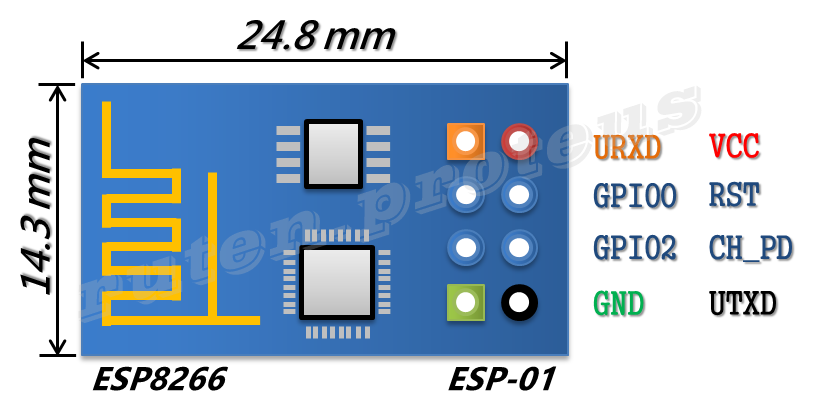
\includegraphics[width=12cm]{images/esp}
  \caption{ESP8266 ESP-01}
  \label{fig:une-autre-image}
\end{figure}

Il m'a fallu décortiquer le SDK pour ré-implémenter une version spécifique minimal du client en C. Cette version expérimental ne pouvait ouvrir qu'un seul websocket de transfert à la fois et le contenu de la page WEB était directement stocké en dur dans le programme du microcontrôleur. Une fois le programme compilé en binaire, il fallait le flashé dans la mémoire FLASH du microcontrôleur en UART (alias Serial), à l'aide d'un adaptateur UART en USB, par exemple de la marque FTDI.

\begin{figure}[htp]
  \centering
  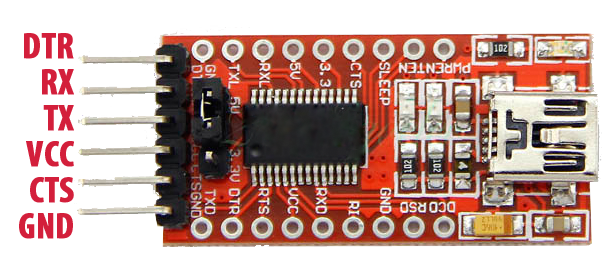
\includegraphics[width=12cm]{images/ftdi}
  \caption{FTDI FT232RL USB to TTL Serial Adapter}
  \label{fig:une-autre-image}
\end{figure}

Ce petit prototype sur microcontrôleur a tout de même était capable de se connecter au serveur par l'intermédiaire de notre WIFI (SSID et mot passe codé en dur dans le programme), son nom de domaine unique généré par le serveur pointait sur la page WEB stocké sur l'ESP, permettant d'allumer/éteindre une LED brancher au microcontrôleur sur le GPIO2 à l'aide d'un bouton HTML.

%%% Local Variables: 
%%% mode: latex
%%% TeX-master: "isae-report-template"
%%% End: 

\chapter*{Conclusion}
\addcontentsline{toc}{chapter}{Conclusion}
\markboth{Conclusion}{Conclusion}
\label{sec:conclusion}

Durant ce stage, j’ai développé le prototype de la solution d'accès distant aux différents services locaux d’un l’objet connecté et plus particulièrement les services WEB liés au protocole HTTP. Pour cela j'ai travaillé sur l'intégralité de la chaîne de développement, j'ai effectué les recherches (pour les choix technologiques), la conception, le développement, la mise en production et bien entendu les tests.

Pour ce projet, j'ai étudié les architectures réseaux des grandes organisations et leurs contraintes ainsi que les différents protocoles nécessaire. J'ai été initié au monde de l'internet des objets, des problèmatiques CLOUD et au monde des microcontrôleur dit industrielle. Les objectifs ont été atteints, toute les fonctionnalités demandés ont été implémenté et testé. Ma solution reste un prototype est devra recevoir une re-mise à niveau pour s'adpater à la solution final qui proposera la société Y3S.

Mon stage m'a permis de m'intégrer dans une entreprise et de m'insérer dans un univers professionnel. J'ai dû acquérir toute les règles de collaboration dans une société. Grâce à mon stage j'ai pu acquérir de solide connaissance en développement réseau sur les sockets natifs, le développement sur plusieurs architectures et l'utilisation de technologies bas niveau en détail avec la programmation sur microcontrôleur et l'implémentation du websocket.

Mon stage m'a conforté dans mon projet professionnel, j'ai souhaite en effet poursuivre mes études pour en apprendre plus sur le développement de technologiques bas niveau, mais orienté dans l'infographie, le son, la vidéo et la 3D.

\chapter*{Webographie}
\addcontentsline{toc}{chapter}{Webographie}
\markboth{Webographie}{Webographie}


\begin{itemize}
\item WebSocket : \\\url{https://developer.mozilla.org/en-US/docs/Web/API/WebSockets_API}\goodbreak\url{/Writing_WebSocket_servers}
\item Node.js : \\\url{https://nodejs.org/en/}
\item Etherws : \\\url{https://pypi.python.org/pypi/etherws/}
\item Node Reverse Wstunnel : \\\url{https://www.npmjs.com/package/node-reverse-wstunnel}
\item Espressif : \\\url{https://espressif.com/en/products/hardware/esp8266ex/overview}
\end{itemize}

%%% Local Variables: 
%%% mode: latex
%%% TeX-master: "isae-report-template"
%%% End: 



\appendix

\bibliographystyle{authoryear-fr}
\bibliography{references}

\end{document}
